\documentclass[11pt]{report}

\usepackage[utf8]{inputenc}
\usepackage[T1]{fontenc}
\usepackage[francais]{babel}

\usepackage{hyperref}
\usepackage{tikz}
\usepackage{amsmath,amssymb}
\usepackage{graphicx}
\usepackage{array}
\usepackage{color}
\usepackage{subfigure}
\usepackage{caption}
\usepackage{booktabs}
\usepackage{threeparttable}
\usepackage{amsmath}
\usepackage{array}
\usepackage{tabularx}
\usepackage{lmodern} % police Latin Modern
\usepackage{hyperref}
\usepackage{fancyhdr}
\usepackage{listingsutf8}
\usepackage{verbatim}
\usepackage[autolanguage]{numprint}
\usepackage{rotating}
\usepackage[top=3cm, bottom=3cm, left=3cm, right=3cm]{geometry}
\pagestyle{fancy}
\addto\captionsfrench{\def\tablename{Tableau}}
\lhead{Stegen Thomas s154315 \quad  Adrien Minne s154340 \quad  Delaunoy Arnaud s153059}
\hypersetup{                    % parametrage des hyperliens
    colorlinks=true,                % colorise les liens
    breaklinks=true,                % permet les retours à la ligne pour les liens trop longs
    urlcolor= black,                 % couleur des hyperliens
    linkcolor= black,                % couleur des liens internes aux documents (index, figures, tableaux, equations,...)
    citecolor= green                % couleur des liens vers les references bibliographiques
    }
\definecolor{mygreen}{RGB}{28,172,0} % color values Red, Green, Blue
\definecolor{mylilas}{RGB}{170,55,241}
\title{Processus stochastiques : cryptanalyse}
\author{Stegen Thomas s154315 \\ Adrien Minne s154340 \\ Delaunoy Arnaud s153059}
\date{}
\renewcommand\thesection{\arabic{section}}
\renewcommand\thesubsection{\arabic{section}.\arabic{subsection}}
\renewcommand\thesubsubsection{Question \arabic{subsubsection}}
\begin{document}
\setcounter{secnumdepth}{3}
\lstset{
language=matlab,
keywordstyle=\color{blue},
morekeywords=[2]{1}, keywordstyle=[2]{\color{black}},
identifierstyle=\color{black},
stringstyle=\color{mylilas},
commentstyle=\color{mygreen},
numberstyle={\tiny \color{black}},
emph=[1]{for,end,break},emphstyle=[1]\color{blue},
}
 \lstset{%
            inputencoding=utf8,
                breaklines=true,
                extendedchars=true,
                literate=%
                {é}{{\'e}}{1}%
                {è}{{\`e}}{1}%
                {à}{{\`a}}{1}%
                {ç}{{\c{c}}}{1}%
                {œ}{{\oe}}{1}%
                {ù}{{\`u}}{1}%
                {É}{{\'E}}{1}%
                {È}{{\`E}}{1}%
                {À}{{\`A}}{1}%
                {Ç}{{\c{C}}}{1}%
                {Œ}{{\OE}}{1}%
                {Ê}{{\^E}}{1}%
                {ê}{{\^e}}{1}%
                {î}{{\^i}}{1}%
                {ô}{{\^o}}{1}%
                {û}{{\^u}}{1}%
                {ë}{{\¨{e}}}1
                {û}{{\^{u}}}1
                {â}{{\^{a}}}1
                {Â}{{\^{A}}}1
                {Î}{{\^{I}}}1
        }

\begin{titlepage}
\maketitle
\end{titlepage}
\section{ Première partie : chaines de Markov pour la modélisation du langage et MCMC}
\subsection{Chaine de Markov pour la modélisation du langage}
\subsubsection{}
L'élément (i,j) de la matrice de transition correspond à la probabilité de passer de l'état i à l'état j. Il correspond donc à la probabilité que la lettre i soit suivie de la lettre j dans la séquence. Dès lors, soit $\theta$ l'élément (i,j) de la matrice de transition, $\theta$ est le paramètre d'une loi de Bernouilli avec comme possibilités:
\begin{itemize}
\item l'élément i est suivi de j (avec une probabilité $\theta$)
\item l'élément i n'est pas suivi de j (avec une probabilité $1-\theta$)
\end{itemize}
\paragraph{}
La méthode du maximum de vraisemblance consiste à maximiser $P(\bf{D}_n|\theta)$ avec $\bf{D}_n$ l'échantillon de donnée, ici seq1 et n le nombre de données. Pour une variable de Bernouilli, on a: Soit,\\ 
$$
\mbox{} x_i = \left\{
    \begin{array}{ll}
        1 & \mbox{si i est suivi de j} \\
        0 & \mbox{si i n'est pas suivi de j}
    \end{array}
\right.
$$
et m le nombre d’occurrences de la lettre i.
\begin{align*}
P(\bf{D}_n|\theta) &= \prod_{i = 1}^{m} (x_i \theta +(1-x_i)(1-\theta)) \\
                   &= \theta^{n_1} (1-\theta)^{n_0}
\end{align*}
Avec $n_0$ le nombre de fois où $x_i = 0$ et $n_1$ le nombre de fois où $x_i = 1$. Déterminons maintenant le $\theta$ maximisant cette fonction:
\begin{align*}
\frac{\partial P(\bf{D}_n|\theta)}{\partial \theta} 
&= n_1 \theta^{n_1-1} (1-\theta)^{n_0} - n_1\theta^{n_1} (1-\theta)^{n_0-1} \\
&= \theta^{n_1-1} (1-\theta)^{n_0-1} (n_1 (1-\theta) - n_0 \theta) \\
&= \theta^{n_1-1} (1-\theta)^{n_0-1} (n_1 - \theta (n_1 + n_0))
\end{align*}
La valeur de $\theta$ maximisant la fonction $P(\bf{D}_n|\theta)$ est donc:
$$ \theta_{i,j} = \frac{n_1}{n_0+n_1} = \frac{\mbox{nombre d'occurrences de i suivies de j}}{\mbox{nombre d'occurrences de i}} $$\\
Ceci est implémenté par la fonction \texttt{transition\_matrix}. Dans le cas de la séquence qui a été fournie,
$$Q =
\begin{bmatrix}
0 & 0.0857 & 0.1000 & 0.8143 \\
1.0000 & 0 & 0 & 0 \\
0.6744 & 0 & 0 & 0.3256 \\
0.3662 & 0.1268 & 0.5070 & 0 \\
\end{bmatrix}
$$ 
Ce qui donne le diagramme d'état repris a la figure \ref{etat}.\\
\begin{figure}[!h]
\begin{center}
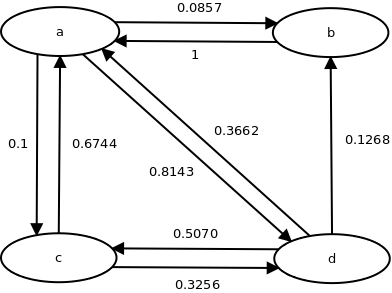
\includegraphics[height = 7cm]{diagramme_etat.png}
\caption{\label{etat}}
\end{center}
\end{figure}
De la même manière, la distribution de probabilité initiale sera calculée de la façon suivante. La probabilité que la chaîne commence par x vaut $\frac{\mbox{nombre de caractères débutant une chaîne valant x}}{\mbox{nombre de caractères débutant une chaîne}}$.\\
Dans ce cas ci, vu qu'il n'y a que une seule chaîne et quelle débute par a,
$$\pi(0) = (1\ 0\ 0\ 0)$$
\subsubsection{}
Cette question est résolue par la fonction \texttt{estimate\_prob}. La t-ième puissance de Q est simplement calculée avec l'opérateur exposant de matlab.\\
Pour le calcul de $P(X_t = x)$, on calcule $\pi(t) = \pi(0)*Q^t$ avec $\pi(0) = (0.25\ 0.25\ 0.25\ 0.25)$ dans le cas ou la première lettre est choisie au hasard et $\pi(0) = (0\ 0\ 1\ 0)$ quand la première lettre est c. $P(X_t = x)$ est l'élément de $\pi(t)$ correspondant à x (le premier pour a, le deuxième pour b, ...).\\
L'évolution de la probabilité est reprise sur les graphiques \ref{prob_a}, \ref{prob_b}, \ref{prob_c} et \ref{prob_d}. On constate qu'en t = 0, elle est uniquement dépendante de $\pi(0)$, ce qui est normal au vu de la définition de $\pi(0)$. Quand t augmente, la probabilité est de moins en moins dépendante de $\pi(0)$ et dépend donc de plus en plus de la matrice de transition. C'est en accord avec la théorie car quand le temps augmente, la distribution tend vers la distribution stationnaire si $Q^t$ converge vers une valeur limite pour $t \rightarrow +\infty$. C'est le cas ici car 
$$Q^{1000} = Q^{1001} =
\begin{bmatrix}
0.3518 & 0.0754 & 0.2161 & 0.3568\\
0.3518 & 0.0754 & 0.2161 & 0.3568\\
0.3518 & 0.0754 & 0.2161 & 0.3568\\
0.3518 & 0.0754 & 0.2161 & 0.3568
\end{bmatrix}
$$ 
\begin{figure}[!h]
\begin{center}
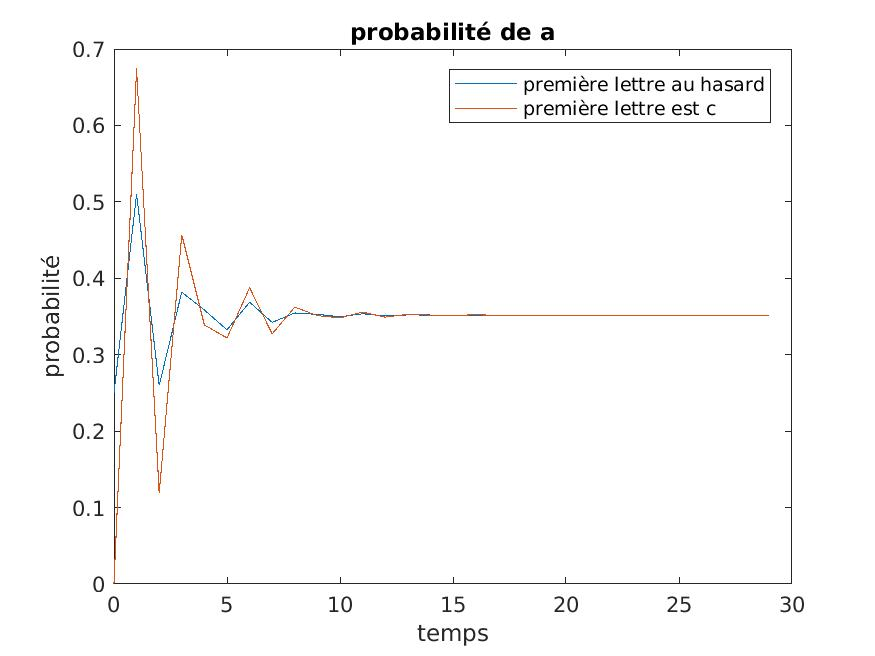
\includegraphics[height = 9cm]{prob_a.jpg}
\caption{\label{prob_a}}
\end{center}
\end{figure}
\begin{figure}[!h]
\begin{center}
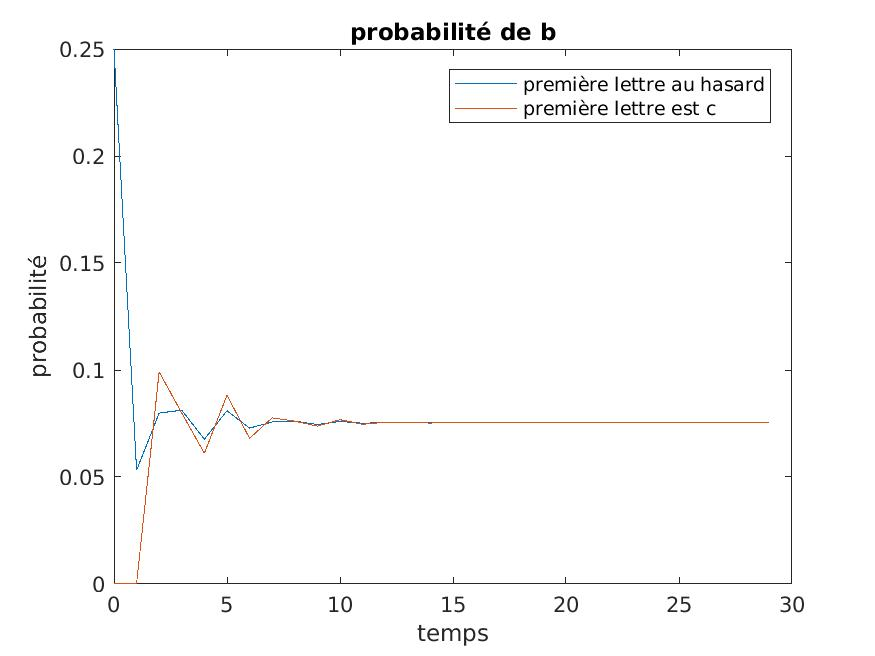
\includegraphics[height = 9cm]{prob_b.jpg}
\caption{\label{prob_b}}
\end{center}
\end{figure}
\begin{figure}[!h]
\begin{center}
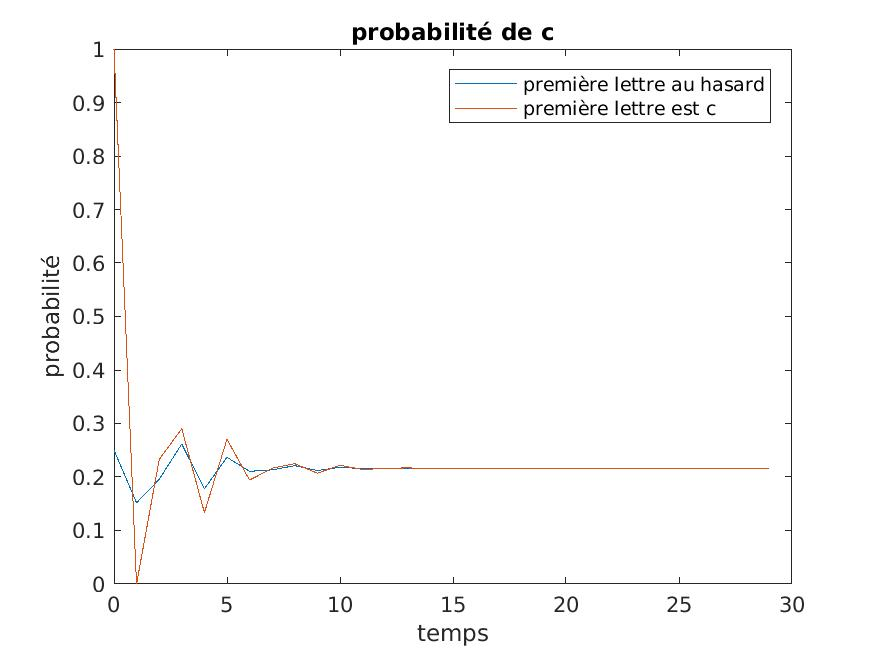
\includegraphics[height = 9cm]{prob_c.jpg}
\caption{\label{prob_c}}
\end{center}
\end{figure}
\begin{figure}[!h]
\begin{center}
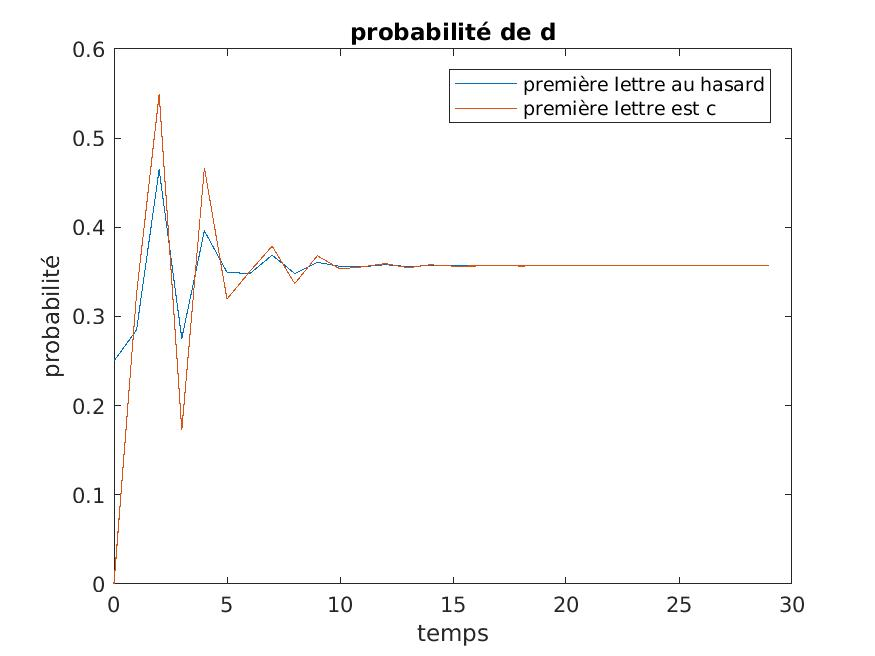
\includegraphics[height = 9cm]{prob_d.jpg}
\caption{\label{prob_d}}
\end{center}
\end{figure}
\subsubsection{}
Cette question est résolue par la fonction \texttt{distrib\_station}. La distribution stationnaire peut être obtenue en multipliant une distribution initiale $\pi(0)$ par la matrice de transition jusqu'à convergence (jusqu'à ce que la différence entre deux itérations soit inférieure à une certaine valeur, qui se doit d'être suffisamment faible). Nous avons utilisé une autre solution équivalent qui consiste à multiplier la matrice de transition par elle-même jusqu'à convergence. La matrice obtenue aura toute ses lignes ayant la même valeur et cette valeur sera la distribution stationnaire.
La distribution stationnaire obtenue est 
$$\pi_{\infty} = (0.3518\ 0.0754\ 0.2161\ 0.3568)$$.
\subsubsection{}
La fonction générant la réalisation de la chaîne de Markov est \texttt{realisation}. Elle est implémentée de cette façon, la première lettre est tirée selon la distribution stationnaire et les suivantes selon la ligne de la matrice Q correspondant à la lettre précédente.\\
Les résultat de la proportion de chaque lettre dans la chaîne de Markov pour des longueurs données sont repris au tableau \ref{Q_114} On constate que pour une longueur de chaîne qui augmente, la proportion de chaque lettre tend vers la distribution stationnaire.
\begin{center}
\begin{threeparttable}
\begin{tabular}{|c|c|c|c|c|}
\hline
longueur & a & b & c & d \\
\hline
1 & 0 & 0 & 0 & 1 \\
\hline
10 & 0.3 & 0 & 0.2 & 0.5 \\
\hline
50 & 0.36 & 0.04 & 0.2 & 0.4 \\
\hline
100 & 0.35 & 0.08 & 0.22 & 0.35 \\
\hline
200 & 0.345 & 0.075 & 0.2 & 0.38 \\
\hline
500 & 0.37 & 0.076 & 0.208 & 0.346 \\
\hline
1000 & 0.347 & 0.08 & 0.215 & 0.358 \\
\hline
10000 & 0.3546 & 0.791 & 0.2125 & 0.3538 \\
\hline
100000 & 0.35248 & 0.07425 & 0.2164 & 0.35687\\ 
\hline
\end{tabular}
\caption{\label{Q_114}proportion dans réalisation de chaîne de Markov}
\end{threeparttable}
\end{center}
\subsubsection{}
Cette expérience permet de montrer que la variance d'échantillon diminue avec la taille de l'échantillon. En effet, plus la taille augmente et plus les résultats trouvé tendent vers l'espérance (la distribution stationnaire).\\
En plus de cette expérience, nous avons testé de faire la moyenne d'un nombre élevé de réalisations de longueur 1. Les proportions tendent également vers la distribution stationnaire. Le fait que ces deux expériences amènent aux mêmes résultats montre que la génération d'un élément dans la chaîne de Markov est indépendant du temps. On est donc en présence d'un processus ergodique. Attention, cette dernière remarque n'est valable que car on démarre de la distribution stationnaire.
\subsection{Algorithme MCMC}
\subsubsection{}
Pour prouver que $\pi_0$ est une distribution stationnaire de la chaine de Markov, il suffit de prouver que $\pi_0=\pi_0 *Q$. 
On sait que les équations de balances détaillées $\pi_0(i)Q_{i,j} = \pi_0(j)Q_{j,i}$ sont satisfaites.
Passant en notation indicielle, on doit donc montrer que :
\begin{align*}
\pi_0(i) &= \sum^{N}_{k=0} \pi_0(k)*Q_{k,i} \\
& = \sum^{N}_{k=0} \pi_0(i)*Q_{i,k} \\
& = \pi_0(i) \sum^{N}_{k=0} \pi_0(i) Q_{i,k} \\
& = \pi_0(i)
\end{align*}
Cette distribution stationnaire est unique si la matrice de transition Q est irréductible.
\subsubsection{}
Cette démonstration a été faite avec l'aide du pdf nommé MetropolisExplanation mis dans l'archive trouvé sur internet.\\
Étudions d'abord la probabilité de transition.\\
La probabilité d'obtenir un élément $x_j$ sachant que l'élément précédent de la chaîne de Markov est $x_i$ est pour $i \neq j$ la probabilité que cet élément soit généré selon la loi q et accepté.
$$P(x_j | x_i) = \alpha(x_j, x_i) q(x_j| x_i)$$
avec
\begin{align*}
\alpha(x_j, x_i) 
&= min \left\{1, \frac{f(x_j)}{f(x_i)} \frac{q(x_i|x_j)}{q(x_j|x_i)}\right\}\\
&= min \left\{1, \frac{cP_X(x_j)}{cP_X(x_i)} \frac{q(x_i|x_j)}{q(x_j|x_i)}\right\}
\end{align*}
La probabilité d'obtenir à nouveau l'élément $x_i$ sachant que l'élément précédent de la chaîne de Markov est également $x_i$ est la somme de la probabilité que l'élément $x_i$ soit généré selon la loi q et accepté et de la probabilité que tout autre élément soit généré et refusé.
$$P(x_i | x_i) = \alpha(x_i, x_i) q(x_i|x_i) + \sum_k (1-\alpha(x_k, x_i)) q(x_k |x_i)$$

Dans le cas où l'élément généré est différent du précédent, on a:
\begin{align*}
P(x_j | x_i) \pi_0(x_i)
&= \alpha(x_j, x_i) q(x_j| x_i) \pi_0(x_i) \\
&= min \left\{1, \frac{cP_X(x_j)}{cP_X(x_i)} \frac{q(x_i|x_j)}{q(x_j|x_i)}\right\} q(x_j| x_i) \pi_0(x_i) \\
&= \frac{\pi_0(x_i)}{cP_X(x_i)} min \left\{cP_X(x_i) q(x_j|x_i), cP_X(x_j) q(x_i|x_j)\right\} \\
&\text{en posant } x_i \leftarrow x_j \text{ et } x_j \leftarrow x_i \\
&= \frac{\pi_0(x_j)}{cP_X(x_j)} min \left\{cP_X(x_j) q(x_i|x_j), cP_X(x_i) q(x_j|x_i)\right\} \\
&= min \left\{1, \frac{cP_X(x_i)}{cP_X(x_j)} \frac{q(x_j|x_i)}{q(x_i|x_j)}\right\} q(x_i| x_j) \pi_0(x_j)\\
&= \alpha(x_i, x_j) q(x_i| x_j) \pi_0(x_j) \\
&= P(x_i | x_j) \pi_0(x_j)
\end{align*} 

Dans le cas où l'élément généré est le même que le précédent, $x_i$ étant égal à $x_j$ il est évident que 
$$P(x_i | x_j) \pi_0(x_j) = P(x_j | x_i) \pi_0(x_i)$$
car 
$$P(x_i | x_i) \pi_0(x_i) = P(x_i | x_i) \pi_0(x_i)$$
\section{Deuxième partie : décryptage d’une séquence codée}
\subsubsection{}
Pour déterminer la cardinalité de l'ensemble $\Theta$, il suffit de calculer le nombre possibles de permutations des caractères disponibles. On considère la langue anglaise avec 40 caractèresle nombre de permutations possibles, on considère qu'on a 40 permutatations possibles pour la première lettre, 39 pour la deuxième, ... On a donc : 
$$|\Theta| = 40 * 39 *38 * ... * 1!$$. 
\subsubsection{}
\paragraph{}
Dans le modèle $\pi_0, Q$, on peut trouver la vraisemblance de la séquence $T'$ en mutlipliant les probabilité d'avoir la lettre $n$ de $T'$ en partant de la lettre $n-1$ de $T'$. Nos probabilités sont calculées comme suit : 

\begin{itemize}
\item $P(lettre 1 = T'(1))$ est simplement sa probabilité d'avoir cette lettre dans $\pi_{0}$.
\item $P(lettre 2 = T'(2))$ : est la probabilité d'avoir cette lettre dans $\pi_{0}*Q$.
\item $P(lettre 3 = T'(3))$ : est la probabilité d'avoir cette lettre dans $\pi_{0}*Q^{2}$.
\item etc
\end{itemize}

La vraisemblance de la chaine $T'$ est donc, notant N la taille de la chaine $T'$ et $| \pi|_{T'(k)}$ la probabilité d'avoir la $k^{ième}$ lettre de $T'$ selon la distribution $\pi$ :
$$P(T') = \prod_{k=0}^{N} |\pi_{0}*Q^{k}|_{T'(k)}$$

\paragraph{}
Pour trouver la vraisemblance de $D$, il faut d'abord calculer la matrice $Q_{\theta}$ exprimant notre matrice Q dans le cas  de la permutation $\theta$. Ensuite, la vraisemblance de $D$ se trouve de la même facon que celle de $T'$, à savoir : 
$$P(D) = \prod_{k=0}^{N} |\pi_{0}*Q_{\theta}^{k}|_{D(k)}$$

\subsubsection{}

Si il n'a que 10 codes candidats possible qui ont la même probabilité, il est assez simple de retrouver le texte de base. Il suffit en effet de calculer la vraisemblance de notre texte avec chaque code $\theta$ suivant l'algorithme décrit au point 2.2, et puis simplmenet sélectionner le $\theta$ menan	t au texte ayant la plus grande vraisemblance.
\subsubsection{}
L'algorithme ayant été implémenter en suivant le pseudo-code donné, nous n'allons discuter que des particularités différentes du pseudo-code et pas l'algorithme dans son ensemble. La fonction implémentant l'algorithme s'appelle \texttt{Metro\_Hast}. \\
Les seules particularités et difficultés de l'algorithme résident dans le calcul des probabilités permettant de calculer $\alpha$.\\
Premièrement, nous considérons $q(x^{(t-1)}|y^{(t)}) = q(y^{(t)}|x^{(t-1)})$. En effet, toutes les fonctions de proposition q que nous utilisons résultent de permutations aléatoires ou sont des fonctions indépendantes de l'état précédent et uniformément distribuées. Le deuxième cas implique logiquement que l'évaluation de tout élément généré par q est le même. Le premier cas implique également cette possibilité car les permutations étant aléatoires, la probabilité de refaire la permutation arrière est la même que celle de faire la permutation qui a été faite pour arriver à cet état.\\
Deuxièmement, en ce qui concerne le calcul de $P_x$,

\subsubsection{}
La distribution de proposition choisie est implémentée par la fonction \texttt{random\_flip} et consiste à permuter la position de deux élément dans la permutation de l'alphabet actuelle. L'expérience menée consiste à exécuter l'algorithme 20 pour chaque longueur traitée. L'algorithme est utilisé avec les caractéristiques suivantes:
\begin{itemize}
\item la permutation de départ est celle ne permutant aucun caractère de la chaîne.
\item la convergence est considérée atteinte après avoir conservé l'ancienne valeur de x 100 fois dans l'algorithme.
\item Si la convergence n'est pas atteinte après 20000 itérations de l'algorithme, l'algorithme s'arrête et on considère qu'il n'y a pas convergence. La qualité de la chaîne produite est tout de même évaluée car on a remarqué expérimentalement que le fait de ne pas atteindre la convergence ne diminue pas la qualité de la chaîne et il n'y a donc pas d'intérêt à différencier ces métriques.
\end{itemize} 
Afin d'évaluer la convergence, les métriques utilisées sont la proportion d'exécution amenant à une convergence (selon les critères définis ci-dessus) et le nombre moyen d'itérations nécessaires à la convergence si il y a convergence.\\

En ce qui concerne la qualité de la chaîne, la métrique utilisée est la proportion de chaîne correctement déchiffrées (convergence ou non). Le pourcentage de chaîne correctement déchiffrées à été obtenu en comparant à un résultat obtenu précédemment que l'on sait correct la chaîne décryptée, en permettant quelques erreurs. En effet, dans le cadre de ce projet, le but est de rendre un texte codé en texte intelligible, et quelques erreurs mineures (par exemple changer les "-" en ";") n'influent pas vraiment notre capacité à comprendre le texte décrypté.
D'un point de vue pratique, les signes de ponctuation "rares" (:, ;, ?, ...), sont problématiques puisque comme ils sont en petit nombres, ils influent beaucoup moins la probabilité de la chaîne par rapport à permuter deux lettres de l'alphabet, et l'algorithme a donc beaucoup plus de mal à converger vers la bonne valeur de ces symboles. Dans notre cas, nous avons par exemple "slow-moving", qui sera décrypté en "slow;moving" ou "slow?moving", mais nous considérons que ça n'affecte pas la compréhension et que ce n'est pas une erreur.\\
Le tableau \ref{Q_225} reprend ces différentes métriques. On remarque que plus la chaîne est longue, plus la convergence est rapide et plus la qualité du résultat obtenu est élevée. C'est assez logique car plus la chaîne est longue, plus on a d'information alors que le nombre d'inconnues reste constant (il y a toujours autant de caractères dans l'alphabet). On pourrait considérer que le nombre d'inconnues n'est pas tout à fait constant car plus la chaîne est courte, plus les chances que des caractères ne soient pas dans la chaîne sont élevées mais c'est négligeable par rapport à l'apport d'information.

\begin{center}
\begin{threeparttable}
\begin{tabular}{|c|c|c|c|c|}
\hline
longueur & \% convergence & nombre d'itérations si convergence & \% correct \\
\hline
10 & 0 & pas applicable & 0 \\
\hline
100 & 0 & pas applicable & 0 \\
\hline
500 & 0 & pas applicable & 45 \\
\hline
750 \\
\hline
1000 \\
\hline
1300 & 80 & 8690 & 60 \\
\hline
\end{tabular}
\caption{\label{Q_225} convergence et qualité selon la longueur d'une chaîne}
\end{threeparttable}
\end{center}
\subsubsection{}
Pour implémenter la convergenace dans notre algorithme, nous avons tout simplement regardé le nombre d'itération successives pour lesquelles l'état courant de notre algorithme de Metropolis-Hastings reste le même. Nous donnons ensuite une valeur x de convergeance à l'algorithme, et quand l'état courant est resté x fois le même, nous considérons que la convergeance est atteinte. \\

Nous avons ensuite conduit une série de test pour regarder les résultats en fonction des différentes valeurs de convergeance. Ces tests ont été effectués avec un nombre limite d'itération de l'algorithme de 20000.\\

Nous voyons dans les tableaux \ref{stats_conv1}, \ref{stats_conv2}, \ref{stats_conv3} et \ref{stats_conv4} que la seule méthode convergeant est \texttt{random\_flip} comme attendu (si arnaud en parle dans le 2.5). On remarque que si la valeur seuil de convergence est trop basse, on convergera trop vite et on n'obitendra pas la bonne réponse. On voit aussi que même pour des valeurs de convergeance assez élevées, les méthodes \texttt{rand}

\begin{table}[!h]
\centering
\begin{tabular}{|c|c|c|c|}
  \hline
  Convergeance & Moyenne itérations & \% convergeance & \% corrects \\
  \hline
  10 & 79.75 & 100 & 0\\
  \hline
  50 & 1137.15 & 100 & 0\\
  \hline
  100 & 9731.7 & 90 & 45 \\
  \hline
  200 & 20000 & 0 & 45 \\
  \hline
  500 & 20000 & 0 & 45 \\
  \hline
\end{tabular}
\caption{\label{stats_conv1} Statistique sur la convergeance de l'algorithme random\_flip }
\end{table}
\begin{table}[!h]
\centering
\begin{tabular}{|c|c|c|c|}
  \hline
  Convergeance & Moyenne itérations & \% convergeance & \% corrects \\
  \hline
  10 & 47.9 & 100 & 0\\
  \hline
  50 & 350.1 & 100 & 0\\
  \hline
  100 & 886.1 & 100 & 0 \\
  \hline
  200 & 2025.7 & 100 & 0 \\
  \hline
  500 & 7319.3 & 100 & 0 \\
  \hline
\end{tabular}
\caption{\label{stats_conv2} Statistique sur la convergeance de l'algorithme random\_flip\_4 }
\end{table}
\begin{table}[!h]
\centering
\begin{tabular}{|c|c|c|c|}
  \hline
  Convergeance & Moyenne itérations & \% convergeance & \% corrects \\
  \hline
  10 & 55.4 & 100 & 0\\
  \hline
  50 & 1708.3 & 100 & 0\\
  \hline
  100 & 4740.8 & 65 & 0 \\
  \hline
  200 & 19902 & 5 & 0 \\
  \hline
  500 & 20000 & 0 & 0 \\
  \hline
\end{tabular}
\caption{\label{stats_conv3} Statistique sur la convergeance de l'algorithme random\_flip\_close }
\end{table}
\begin{table}[!h]
\centering
\begin{tabular}{|c|c|c|c|}
  \hline
  Convergeance & Moyenne itérations & \% convergeance & \% corrects \\
  \hline
  10 & 17.3 & 100 & 0\\
  \hline
  50 & 89.3 & 100 & 0\\
  \hline
  100 & 163.45 & 100 & 0 \\
  \hline
  200 & 356.1 & 100 & 0 \\
  \hline
  500 & 946.5 & 100 &  0\\
  \hline
\end{tabular}
\caption{\label{stats_conv4} Statistique sur la convergeance de l'algorithme random\_permutation }
\end{table}
\end{document}